\section{Theorie}
\label{sec:Theorie}
Wenn auf Festkörper Kräfte einwirken, können Volumen- und Gestaltsänderungen eben dieses Körpers auftreten.
Die Proportionalitätsfaktoren, welche den Zusammenhang zwischen pro Flächenstück einwirkender Kraft und Volumen- bzw. Gestaltänderung beschreiben, werden elastische Konstanten genannt.
Es findet jedoch eine Kathegorisierung der verschiedenen Kräfte in zwei Gruppen statt.\\
Die erste Gruppe stellen Kräfte dar, welche auf ein Volumenelement wirken.
Diese erzeugen eine Änderung des Bewegungszustandes, was in diesem Protokoll nicht weiter behandelt wird.\\
Die Kräfte, welche von Interesse sind, sind die, die auf die Oberfläche eines Körpers wirken und somit eine Gestaltsänderung hervorrufen.
Dabei wird der Kraftbezeichnung zumeist an die Fläche gebunden.
Es entsteht der Begriff der Spannung $([\frac{\text{Kraft}}{\text{Fläche}}])$.
Es wird weiterhin zwischen der Normalspannung $\sigma$, die Spannung die senkrecht an der Oberfläche angreift, und der Schubspannung $\tau$, welche tangential an der Oberfläche wirkt, unterschieden.
Die Auswirkungen beider sind an jeder Querschnittsfläche des Körpers nachweisbar.\\
Wenn der Körper nach der Krafteinwirkung wieder in seinen Ausgangszustand zurückkehrt ist die Rede von elastischer Deformation.
Bei kleinen Auslenkungen besteht ein linearer Zusammenhang zwischen Volumen- bzw. Längenänderung und Druck bzw. Normalspannung, welcher als Hooksches Gesetz bekannt ist.
Dieser Auslenkungsvorgang lässt sich leicht am Beispiel eines Atomgitters verstehen, bei dem alle Atome durch elektrostatische Kräfte in eine Gleichgewichtslage $r_0$ gezwungen werden.
Bei gewissen kleinen Auslenkungen, $r_0 \rightarrow r_0'$, kehrt das Atom wieder in seine ursprüngliche Gleichgewichtslage zurück; ein reversibler Prozess.
Bei größeren Auslenkungen stellt sich eine neue Ruhelage ein.\\
Die elastischen Konstanten von Körpern sind im Allgemeinen richtungsabhängig.
Es ergeben sich insgesamt einundzwanzig Konstanten.
Je höher die innere Symmetrie des Körpers jedoch ist, umso weniger richtungsunabhängig ist die Elastizitätseigenschaft und umso eher isotrop ist das untersuchte Material.
Im Folgenden werden der Praxis halber nur isotrope Materialien näher untersucht.\\
Dort sind generell zwei Konstanten relevant.
Zum Einen der Schubmodul $G$, welcher die Gestaltelastizität beschreibt, und zum Anderen das Kompressionsmodul $Q$, das die Volumenelastizität schildert.
Um die Zusammenhänge besser beschreiben zu können, werden zwei zusätzliche Größen eingeführt.
Die erste ist der Elastizitätsmodul $E$, welcher als Proportionalitätsfaktor zwischen relativer Längenänderung und Normalspannung fungiert.
\begin{equation}
  \sigma = E \frac{\increment L}{L}
\end{equation}
Die zweite ist die Poissonsche Querkontraktionszahl $\mu$, welche die Maßänderungen senkrecht zur Normalspannungsrichtung beschreibt bezogen auf die Breite $B$ und die Länge $L$ des Körpers,
\begin{equation}
  \mu = - \frac{\increment B}{B} \frac{L}{\increment L}.
\end{equation}
Zwischen den vier genannten Größen besteht die beiden Zusammenhänge
\begin{equation}
  E = 2G(\mu+1) \label{eqn:1}
\end{equation}
und
\begin{equation}
  E = 3(1-2\mu)Q. \label{eqn:2}    % Hihi, Muh Kuh xD
\end{equation}
Experimentell kann der Schubmodul $G$ beispielsweise über die durch eine Tangentialspannung $\tau$ entstehende Scherung eines Quaders über den Scherungswinkel $\alpha$, dargestellt in Abbildung \ref{fig:1}, bestimmt werden,
\begin{figure}[H]
  \centering
  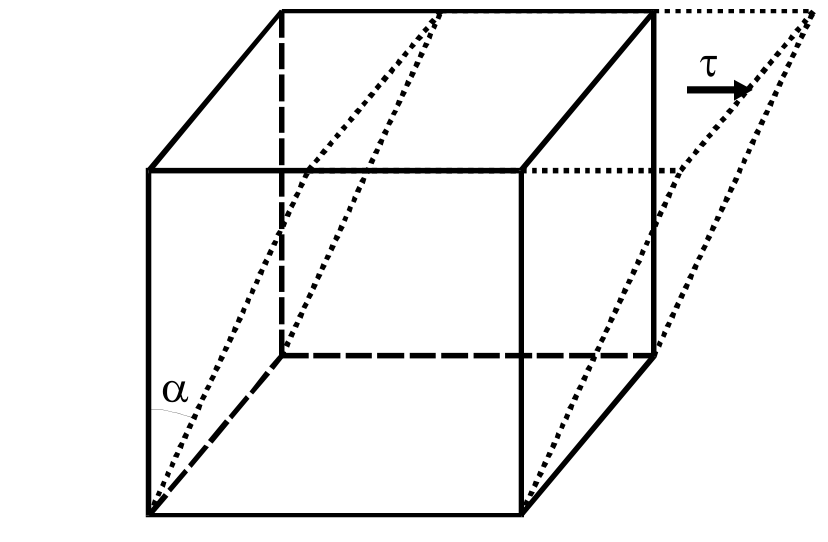
\includegraphics[height=6cm]{scherung1.png}
  \caption{Scherung eines Quaders durch eine Tangentialspannung $\tau$. \cite{sample}}
  \label{fig:1}
\end{figure}
da in diesem Fall
\begin{equation}
  \tau = G \alpha \label{eqn:3}
\end{equation}
gilt.
Weil der Scherungswinkel jedoch schwer zu messen ist, wird der Schubmodul über Torsion bestimmt.
Der Probekörper, praktischerweise in Drahtform bzw. dünner zylindrischer Form, wird dabei wie in Abbildung \ref{fig:2} an einem Ende fest eingespannt, während am anderen zwei Kräfte entgegengesetzt so angreifen, dass der Körper verdrillt wird.
\begin{figure}[H]
  \centering
  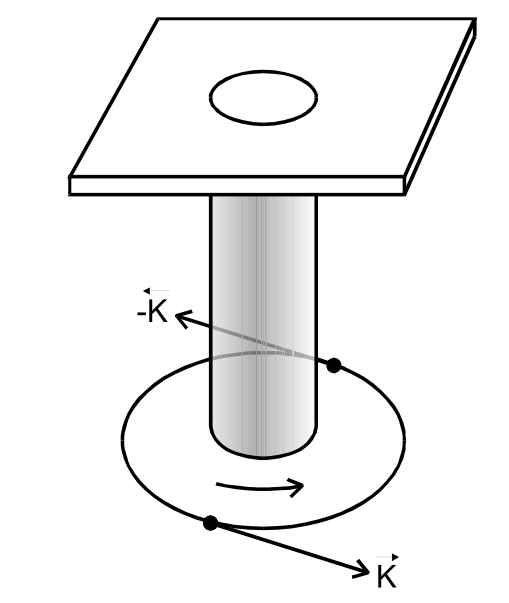
\includegraphics[height=6cm]{scherung2.png}
  \caption{Verdrillung des Körpers. \cite{sample}}
  \label{fig:2}
\end{figure}
Die Mantelfäche des Körpers schert sich nun unter einem Winkel $\alpha$. Diesen Sachverhalt verdeutlicht die Abbildung \ref{fig:3}.
\begin{figure}[H]
  \centering
  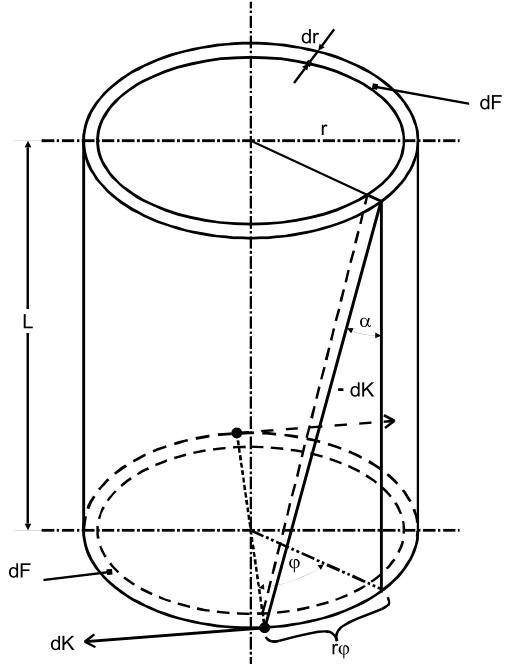
\includegraphics[height=6cm]{scherung3.png}
  \caption{Veranschaulichung der Auswirkung der Verdrillung. \cite{sample}}
  \label{fig:3}
\end{figure}
Es entsteht ein Drehmoment $M$, welches mit dem Winkel $\phi$ über
\begin{equation}
  M_T = \frac{\pi R^4 G}{2L} \phi = D \phi \label{eqn:4}
\end{equation}
den Zusammenhang zum Schubmodul $G$ herstellt.
Dabei ist $R$ der Radius des Zylinders und $L$ dessen Länge.
Der somit definierte Proportionalitätsfaktor $D$ wird als Richtgröße des Zylinders bezeichnet.
Bei diesem Verfahren entsteht aber eine unerwünschte elastische Nachwirkung, welche das nicht instantane Einstellen einer neuen Ruhelage während bzw. nach der Deformation bezeichnet.
Um dies zu verhindern wird eine dynamische Methode gewählt, bei der das Torsionssystem durch einee frei schwingendee Kugel (bezogen auf Torsionsschwingungen) der Trägheit $\theta$ am nicht eingespannten Ende angehängt wird.
Es herrscht nun zusätzlich zum in Gleichung (\ref{eqn:4}) genannten Drehmoment ein neues durch die Trägheit der angehängten Kugel hervorgerufenes Drehmoment.
Es folgt die Differentialgleichung
\begin{equation}
  D \phi + \theta \frac{\symup{d}²\phi}{\symup{d}t²} = 0.
\end{equation}
Dessen Lösung
\begin{equation}
  \phi (t) = \phi_0\cos\left(\frac{2\pi}{T}t\right). \label{eqn:5}
\end{equation}
mit
\begin{equation}
  T = 2\pi\sqrt{\frac{\theta}{D}} \label{eqn:6}
\end{equation}
lautet.
Über das Trägheitsmoment $\theta$ der Kugel,
\begin{equation}
  \theta = \frac{2}{5}m_k R_k^2, \label{eqn:6}
\end{equation}
folgt schließlich
\begin{equation}
  G = \frac{16}{5}\pi\frac{m_k R_k^2 L}{T²R^4}. \label{eqn:7}
\end{equation}
Der Elastizitätsmodul $E$ hingegen wird über die Schallgeschwindigkeit, die im Material herrscht bestimmt, da der Zusammenhang
\begin{equation}
  c² = \frac{E}{\rho},
\end{equation}
mit der Dichte $\rho$ des Materials, besteht.
Aus dem Schub- und Elastizitätsmodul lassen sich nun über (\ref{eqn:1}) und (\ref{eqn:2}) der Kompressionsmodul $Q$ und die Poissonsche Querkontraktionszahl $\mu$ bestimmen.
